\section{Gestion des projets}

\section*{Consultant}

\begin{center}
\scalebox{0.7}{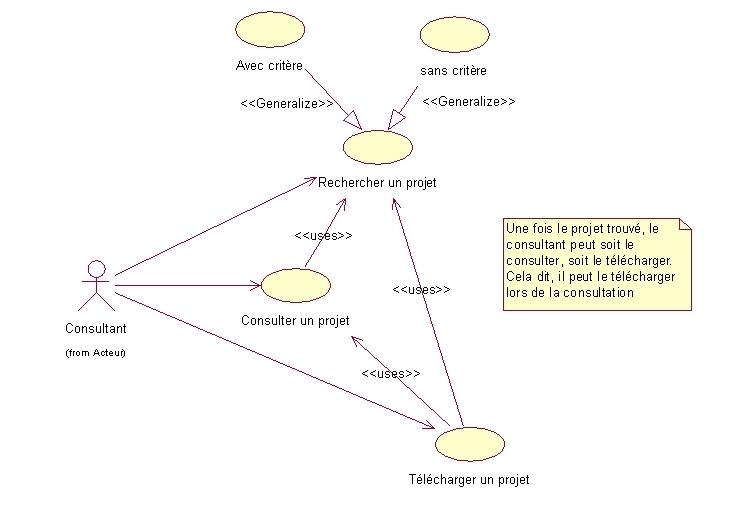
\includegraphics{images/Projet_Consultant.jpg}}\\
\end{center}

\begin{tabular}{|p{4cm}|c|p{4cm}|p{5cm}|}
\hline
Fonction & Priorit{\'e} & Qualit{\'e} & Mesure \\
\hline
Rechercher un projet & 4 & rapide et pr{\'e}cis & La recherche doit {\^e}tre efficace.\\
\hline
Consulter un projet & 5 & rapide et clair & la lisibilit{\'e} de projet doit {\^e}tre facile et agr{\'e}able {\`a} lire.\\
\hline
T{\'e}l{\'e}charger un projet & 2 & fiable et rapide & Le temps de t{\'e}l{\'e}chargement ne doit pas {\^e}tre {\'e}lev{\'e}.\\
\hline
\end{tabular}

\begin{center}
{\'e}chelle de mesure de la priorit{\'e}:

\scalebox{0.5}{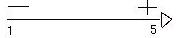
\includegraphics{images/echelle.jpg}}
\end{center}

\begin{itemize}
\item  {\bf Rechercher un projet :}
	\begin{itemize}
	\item Pr{\'e}-requis : Il faut qu'il y ait au moins un projet de cr{\'e}{\'e}.
	\item Description : Il saisie les mots clefs de sa recherche s'il en a dans la case {\it Mots clefs}.\\
	Il valide l'option {\it Recherche} et une liste de projet qui r{\'e}pondent {\`a} sa recherche apparait
	\item Post-requis : La saisie de mot clefs est optionnel, Si aucun mot clef n'est saisie, la recherche liste l'ensemble des projets.\\
	La liste de projet trouv{\'e}s peut contenir de z{\'e}ro {\`a} plusieurs projets.\\
	\end{itemize}

\item  {\bf Consulter un projet :}
	\begin{itemize}
	\item Pr{\'e}-requis :Il faut qu'il y ait au moins un projet de cr{\'e}{\'e}.
	\item Description : Il s{\'e}lectionne successivement les liens lui permettant d'atteindre un projet (ou par recherche).\\
	Il clique pour le visualiser.
	\item Post-requis : Le projet s{\'e}lectionn{\'e} est affich{\'e} au format HTML.\\
	\end{itemize}
			
\item  {\bf T{\'e}l{\'e}charger un projet :}
	\begin{itemize}
	\item Pr{\'e}-requis :Il faut qu'il y ait au moins un projet de cr{\'e}{\'e} et que l'utilisateur ait s{\'e}lectionn{\'e} un projet.
	\item Description : Il s{\'e}lectionne successivement les liens lui permettant d'atteindre un projet (ou par recherche).\\
	L'utilisateur clique l'option {\it T{\'e}l{\'e}charger}, il s{\'e}lectionne l'emplacement sur son compte pour copier le projet et valide.
	\item Post-requis : Le projet est copi{\'e} sur le compte du consultant.\\
	\end{itemize}
\end{itemize}

\section*{Responsable}

\begin{center}
\scalebox{0.7}{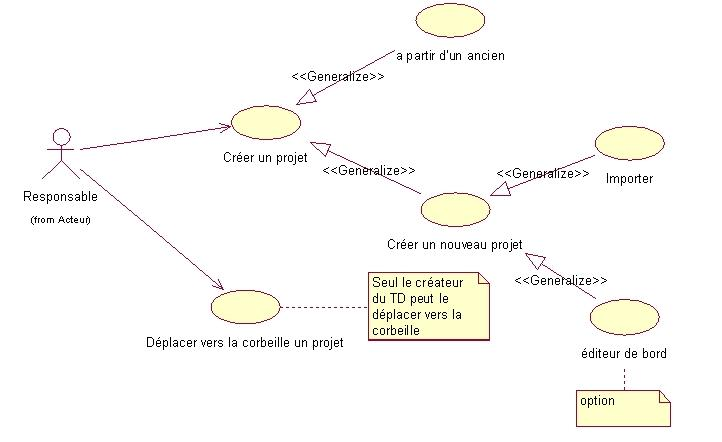
\includegraphics{images/Projet_Responsable.jpg}}\\
\end{center}

\begin{tabular}{|p{4cm}|c|p{4cm}|p{5cm}|}
\hline
Fonction & Priorit{\'e} & Qualit{\'e} & Mesure \\
\hline
Cr{\'e}er un projet & 5 & facile & Doit {\^e}tre facile d'utilisation.\\
\hline
D{\'e}placer vers la corbeille & 2 & fiable & il ne doit pas y avoir de perte d'information.\\
\hline
\end{tabular}
\begin{center}
{\'e}chelle de mesure de la priorit{\'e}:

\scalebox{0.5}{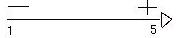
\includegraphics{images/echelle.jpg}}
\end{center}

\begin{itemize}
\item  {\bf Cr{\'e}er un projet :}
	\begin{itemize}
	\item Pr{\'e}-requis : Etre identifi{\'e}.
	\item Description : Il s'identifie avec son login et son mot de passe.\\
	Il s{\'e}lectionne le lien lui permettant de se diriger vers la page de cr{\'e}ation du projet.\\
	Il s{\'e}lectionne l'enseignement pour lequel le projet est destin{\'e}.\\
	Il choisit s'il cr{\'e}e compl{\'e}tement un nouveau projet ou s'il se sert d'un ancien projet :
	\begin{itemize}
		\item : S'il cr{\'e}e un nouveau projet : Il saisie les mots clefs qui serviront pour la recherche de ce projet.\\
		Il s{\'e}lectionne un  exercice dans une liste d'exercices pr{\'e}-enregistr{\'e}s ou il l'importe.
		\item : S'il se sert d'un ancien projet : Le nouveau projet est une copie de l'ancien et l'utilisateur peut alors le modifier.\\
		L'utilisateur peut alors modifier.
	\end{itemize}
	Il valide ses choix.
	\item Post-requis : Un projet ne peut contenir qu'un seul exercice.\\  
	Un nouveau projet est enregistr{\'e} dans la liste des projets disponibles.\\
	\end{itemize}

\item  {\bf D{\'e}placer vers la corbeille :}
	\begin{itemize}
	\item Pr{\'e}-requis : Etre identifi{\'e}.\\
	Il faut qu'au moins un projet soit enregistr{\'e}.\\
	Il doit {\^e}tre le cr{\'e}ateur du projet.
	\item Description : Il s'identifie avec son login et son mot de passe. L'utilisateur doit acc{\'e}der au projet gr{\^a}ce {\`a} la recherche.\\
	Il clique l'option {\it Mettre dans la corbeille}. Il valide sa demande.
	\item Post-requis : le projet est d{\'e}plac{\'e} dans la corbeille.\\
	\end{itemize}
\end{itemize}

\section*{Administrateur}

\begin{center}
\scalebox{0.7}{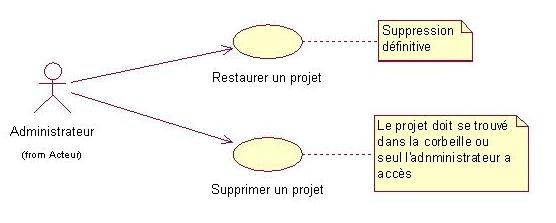
\includegraphics{images/Projet_Administrateur.jpg}}\\
\end{center}

\begin{tabular}{|p{4cm}|c|p{4cm}|p{5cm}|}
\hline
Fonction & Priorit{\'e} & Qualit{\'e} & Mesure \\
\hline
Supprimer un projet & 2 & fiable & Il doit corresponde au fichier selectionn{\'e} pour le supprimer (il ne doit y avoir d'erreur).\\
\hline
Restaurer un projet & 2 & fiable & Il ne doit pas y avoir de perte d'information.\\
\hline
\end{tabular}

\begin{center}
{\'e}chelle de mesure de la priorit{\'e}:

\scalebox{0.5}{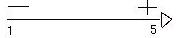
\includegraphics{images/echelle.jpg}}
\end{center}

\begin{itemize}
\item  {\bf Supprimer un projet :}
	\begin{itemize}
	\item Pr{\'e}-requis : Etre identifi{\'e}.\\
	Le projet doit se trouver dans la corbeille.
	\item Description : Il s'identifie avec son login et son mot de passe.\\
	Il affiche les fichiers contenus dans la corbeille. Il s{\'e}lectionne le projet qu'il d{\'e}sire supprimer.\\
	Il clique sur l'option {\it Suppression} et il valide sa s{\'e}lection.
	\item Post-requis : Le projet est supprim�.\\
	\end{itemize}

\item  {\bf Restaurer un projet :}
	\begin{itemize}
	\item Pr{\'e}-requis : Etre identifi{\'e}.\\
	Il faut qu'au moins un projet soit dans la corbeille.
	\item Description : Il s'identifie avec son login et son mot de passe.\\
	Il affiche les fichiers contenus dans la corbeille. Il s{\'e}lectionne le projet qu'il d{\'e}sire restaurer.\\
	Il clique l'option {\it Restaurer} et il valide sa s{\'e}lection.
	\item Post-requis : le projet est d{\'e}plac{\'e} de la corbeille {\`a} l'emplacement qu'il occupait avant d'{\^e}tre plac{\'e} dans la corbeille.\\
	\end{itemize}
\end{itemize}
